% !TeX program = XeLaTeX
% !TeX encoding = UTF-8 Unicode
%
% 为了得到最佳的排版结果,可以考虑安装免费的思源宋体、思源黑体与 M+ 字体
% - 思源字库可以前往
%   https://github.com/adobe-fonts/source-han-serif/tree/release
%   https://github.com/adobe-fonts/source-han-sans/tree/release
% 下载,请安装 Language-specific OTFs 的简体中文版本
% - M+ 字体可以前往
%   https://osdn.net/projects/mplus-fonts/releases/
% 下载
%
% 如果已经安装了思源、M+ 字体,请在导言区启用 \SourceHanSCandMplustrue
%
\documentclass[zihao=5,a4paper]{ctexart}
\XeTeXgenerateactualtext=1 %
\newif\ifSourceHanSCandMplus
\SourceHanSCandMplusfalse
% 如果已经安装了思源、M+ 字体,请启用 \SourceHanSCandMplustrue
%\SourceHanSCandMplustrue
\frenchspacing
\ctexset{
  section={
    name={第,节},
    aftername=\hskip\ccwd\relax,
    format=\Large\bfseries
  },
  subsection/aftername=\hskip\ccwd\relax,
  subsubsection/aftername=\hskip\ccwd\relax
}
\renewcommand\sectionmark[1]{%
  \markright{%
    \normalfont\sffamily
    \CTEXifname{\CTEXthesection\hskip\ccwd\relax}{}#1%
  }%
}
\usepackage{mathtools}
\usepackage[math-style=ISO]{unicode-math}
\ifSourceHanSCandMplus
  \setmainfont{texgyrepagella}[
    Extension=.otf,
    UprightFont=*-regular,
    ItalicFont=*-italic,
    BoldFont=*-bold,
    BoldItalicFont=*-bolditalic,
    Scale=1.05924855491329480,
    SmallCapsFeatures={LetterSpace=5}
  ]
  \setsansfont{texgyreheros}[
    Extension=.otf,
    UprightFont=*-regular,
    ItalicFont=*-italic,
    BoldFont=*-bold,
    BoldItalicFont=*-bolditalic,
    Scale=1.00685871056241427
  ]
  \setmonofont{mplus-1m-regular.ttf}[
    BoldFont=mplus-1m-bold.ttf
  ]
  \setmathfont{texgyrepagella-math.otf}[
    Scale=1.05924855491329480
  ]
  \setCJKmainfont{SourceHanSerifSC-Medium.otf}[
    ItalicFont=SourceHanSerifSC-Heavy.otf,
    BoldFont=SourceHanSerifSC-Bold.otf,
    Language=Chinese Simplified
  ]
  \setCJKsansfont{SourceHanSansSC-Regular.otf}[
    BoldFont=SourceHanSansSC-Bold.otf,
    Language=Chinese Simplified
  ]
  \setCJKmonofont{SourceHanSansSC-Regular.otf}[
    BoldFont=SourceHanSansSC-Bold.otf,
    Language=Chinese Simplified
  ]
  \makeatletter
  \def\setCJKecglue@nnn#1#2#3{%
    \xeCJKsetup
      { xCJKecglue = {\hskip #1em plus #2em minus #3em\relax} }%
  }
  \newcommand*\setCJKecglue{%
    \ifnum\strcmp{\f@family}{\rmdefault}=0 %
      \setCJKecglue@nnn{0.22203274215552524}
                       {0.11101637107776262}
                       {0.07401091405184175}%
    \else
      \ifnum\strcmp{\f@family}{\sfdefault}=0 %
        \setCJKecglue@nnn{0.21859400544959128}
                         {0.10929700272479564}
                         {0.07286466848319709}%
      \else
        \setCJKecglue@nnn{0.25}
                         {0.125}
                         {0.08333333333333333}%
      \fi
    \fi
  }
  \makeatother
  \usepackage{everysel}
  \EverySelectfont{\setCJKecglue}
\else
  \setmainfont{texgyrepagella}[
    Extension=.otf,
    UprightFont=*-regular,
    ItalicFont=*-italic,
    BoldFont=*-bold,
    BoldItalicFont=*-bolditalic,
    SmallCapsFeatures={LetterSpace=5}
  ]
  \setsansfont{texgyreheros}[
    Extension=.otf,
    UprightFont=*-regular,
    ItalicFont=*-italic,
    BoldFont=*-bold,
    BoldItalicFont=*-bolditalic
  ]
  \setmathfont{texgyrepagella-math.otf}
\fi
\usepackage{zhlineskip}
\SetTextEnvironmentSinglespace{1.05}
\SetMathEnvironmentSinglespace{1.05}
\ifSourceHanSCandMplus
  \SetTextEnvironmentSinglespace{1.112}
  \SetMathEnvironmentSinglespace{1.112}
\fi
\usepackage{caption}
\DeclareCaptionLabelFormat{zhlabel}{\bothIfFirst{#1}{\nobreak\CJKecglue}#2\CJKecglue}
\DeclareCaptionLabelSeparator{zhcolon}{\char"FF1A }% Fullwidth Colon
\captionsetup{format=hang,labelformat=zhlabel,labelsep=zhcolon,font={small,sf}}
\usepackage{enumitem}
\setlist{
  listparindent=\parindent,parsep=\parskip
}
\ifSourceHanSCandMplus
  \setlist[itemize,1]{
    itemsep=0pt,
    label=\char"30FB,% Katakana Middle Dot
    leftmargin=\parindent,labelsep=0pt,labelwidth=0.5\parindent
  }
\else
  \setlist[itemize,1]{
    itemsep=0pt,
    label=\char"00B7,% Middle Dot
    leftmargin=\parindent,labelsep=0pt,labelwidth=0.5\parindent
  }
\fi
\setlist[description,1]{
  font=\bfseries,
  leftmargin=\parindent,labelsep=0.5\parindent
}
\usepackage{booktabs}
\usepackage{hyperref}
\hypersetup{
  colorlinks=true,
  pdfstartview={FitH},
  unicode=true,
  pdftitle={zhlineskip},
  pdfauthor={Ruixi Zhang}
}
\usepackage[open,openlevel=-1,numbered]{bookmark}
\usepackage[text={378bp,609bp},centering]{geometry}

\makeatletter
\ExplSyntaxOn
\ifSourceHanSCandMplus
  \xeCJK_new_class:n { PoZheHao }
  \__xeCJK_save_CJK_class:n { PoZheHao }
  \seq_map_inline:Nn \g__xeCJK_class_seq
    {
      \str_if_eq:nnF {#1} { PoZheHao }
        {
          \xeCJK_copy_inter_class_toks:nnnn { PoZheHao } {#1} { FullRight } {#1}
          \xeCJK_copy_inter_class_toks:nnnn {#1} { PoZheHao } {#1} { FullRight }
        }
    }
  \xeCJK_declare_char_class:nn { PoZheHao } { "2014 , "2015 }
\fi
\ExplSyntaxOff
% From `doc.dtx'
\ifx\l@nohyphenation\undefined
  \newlanguage\l@nohyphenation
\fi
\newcommand*\meta{}
\DeclareRobustCommand\meta[1]{%
     \ensuremath\langle
     \ifmmode \expandafter \nfss@text \fi
     {%
      \meta@font@select
      \edef\meta@hyphen@restore
        {\hyphenchar\the\font\the\hyphenchar\font}%
      \hyphenchar\font\m@ne
      \language\l@nohyphenation
      #1\/%
      \meta@hyphen@restore
     }\ensuremath\rangle
}
\def\meta@font@select{\itshape}
% From `ltxdoc.dtx'
\newcommand*\cmd[1]{\cs{\expandafter\cmd@to@cs\string#1}}
\def\cmd@to@cs#1#2{\char\number`#2\relax}
\newcommand*\cs{}
\DeclareRobustCommand\cs[1]{\texttt{\char`\\#1}}
\newcommand\marg[1]{%
  {\ttfamily\char`\{}\meta{#1}{\ttfamily\char`\}}}
\newcommand\oarg[1]{%
  {\ttfamily[}\meta{#1}{\ttfamily]}}
\newcommand\parg[1]{%
  {\ttfamily(}\meta{#1}{\ttfamily)}}
% My commands
\newcommand\cls[1]{{\ttfamily#1}}
\newcommand\pkg[1]{{\ttfamily#1}}
\newcommand\opt[1]{{\ttfamily#1}}
\newcommand\env[1]{{\ttfamily#1}}
\newcommand*\packagedependency[1]{%
  \mbox{\pkg{#1}\CJKecglue 宏包:}\ignorespaces
}
\newcommand*\keyvalueitem[3][2.5]{%
  \item[\opt{#2}\hskip0.5\ccwd\relax\rlap{\meta{#3}}\hskip#1\ccwd\relax]%
  \hskip\z@ \@plus 0.25\ccwd \@minus 0.25\ccwd
  \ignorespaces
}
\newcommand*\usercmditem[3][3]{%
  \item[\cmd{#2}\rlap{\marg{#3}}\hskip#1\ccwd\relax]%
  \hskip\z@ \@plus 0.25\ccwd \@minus 0.25\ccwd
  \ignorespaces
}
\newcommand*\defaultleadingratio[3]{%
  \opt{#1} & $#2$ & $#3$%
}
\newcommand*\fontandsinglespaceratio[2]{%
  #1 & $#2$%
}
\newenvironment{originalpmatrix}{\left(\env@matrix}{\endmatrix\right)}
\newenvironment{originalcases}{\env@cases}{\endarray\right.}
\newcounter{example}
\newcommand*\example{%
  \refstepcounter{example}%
  例\nobreak\CJKecglue\theexample\CJKecglue\char"FF1A %
}
\newenvironment{english}
  {\addvspace\medskipamount}
  {\par\addvspace\medskipamount}
\newcommand*\myemail{ruixizhang42@gmail.com}
\makeatother

\title{\vspace*{-26bp}\pkg{zhlineskip} 宏包}
\author{张瑞熹\thanks{\href{mailto:\myemail}{\nolinkurl{\myemail}}。}}
\date{2019/05/15\hskip\ccwd\relax v1.0e}

\begin{document}

\maketitle

\tableofcontents

\section{简介}

\pkg{zhlineskip} 宏包允许用户指定正文行距相比于正文字号的倍数(通常建议设置在
$1.5$ 至 $1.67$ 之间),以及脚注行距相比于脚注字号的倍数。另一方面,由于数学公式
主要是由西文字符构成的,\pkg{zhlineskip} 还能将数学公式的行距“恢复”成西文
较为紧凑的行距(通常为西文字号的 $1.2$\nobreak\CJKecglue 倍),使得全文的视觉
密度较为均匀。最后,本宏包还支持按照 Microsoft Word 进行“多倍行距”排版。

\subsection{宏包依赖}

本宏包是针对中日韩文的横排文档设计出来的,它依赖于下面这些宏包:
\begin{itemize}
\item \packagedependency{kvoptions}
为用户提供载入本宏包的键值选项。
\item \packagedependency{xintexpr~}
实现精确的浮点运算,属于\CJKecglue\pkg{xint} 宏集的一个部分。
\item \packagedependency{etoolbox~}
处理脚注行距与数学行距时需要打补丁。
\item \packagedependency{mathtools}
只有在恢复数学行距为西文行距时,才会载入这个宏包。
\end{itemize}
请确保你的 \TeX\ 发行版里已经安装好了以上这些宏包的最新版本。

\subsection{中西有别}

在西文排版里,相邻两行\emph{基线}(baseline)之间的距离称为\emph{行距}(leading,
发音为 led-ding)。这个词的词根是 lead,即\emph{铅}。早在铅字时代,每当工匠填满
一行铅字之后要开始填下一行,都会在两行之间插入铅条,从而适当地扩大行距。因为西文的
每个字母四周与其\emph{字框}(em-box,见图\nobreak\CJKecglue\ref{fig:eng-font-size})之间有
较大的空隙,所以不需要插入很高的铅条。一般来说,西文的行距为\emph{字号}(font
size)的 $1.2$ 至 $1.45$\nobreak\CJKecglue 倍\footnote{参见
\url{https://practicaltypography.com/line-spacing.html}。}。

\begin{figure}[h]
\centering

\includegraphics{Latinmetrics}
\caption[西文字体]{西文字体。绿色方框即为 em-box,它在纸上的实际边长就是西文字号。}
\label{fig:eng-font-size}
\end{figure}

中文排版虽然没有基线的概念,但有非常相似的概念:\emph{底线}(ideographic baseline,
见图\nobreak\CJKecglue\ref{fig:chi-font-size})。中文里相邻两行底线之间的距离,与西文里行距的
概念是一致的。另一概念是上一行底线和下一行\emph{顶线}之间的距离,即\emph{行间距}(line
gap),这与西文里插入铅条的高度是一致的。由于汉字四周与其字框间的空隙较小,所以需要
使用比西文更大的行间距。根据场合不同,行间距从字号的 $1/4$ 至 $1$\nobreak\CJKecglue 倍不等:以中文
书刊为例,行间距一般为字号的 $1/2$ 至 $2/3$\nobreak\CJKecglue 倍\footnote{参见张胜涛、王忆波著
《方正飞腾4.0实用培训教程》,第\nobreak\CJKecglue6.1.1\nobreak\CJKecglue 节。},即行距约为字号的
$1.5$ 至 $1.67$\nobreak\CJKecglue 倍。

\begin{figure}[h]
\centering
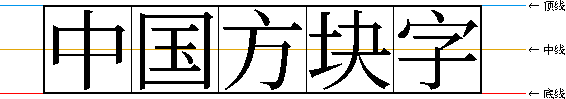
\includegraphics{CJKmetrics}
\caption[中文字体]{中文字体。汉字字面几乎占满整个字框,字框的边长即为中文字号。}
\label{fig:chi-font-size}
\end{figure}

在一般情况下,\CTeX\ 会默认用\CJKecglue\opt{linespread=1.3} 这个文档类
选项将中文的行距设置为字号的 $1.56$\nobreak\CJKecglue 倍(基础行距是字号的
$1.2$\nobreak\CJKecglue 倍,而 $1.2 \times 1.3
= 1.56$)。通过这种方法扩大全文的行距,自然会影响到文章里数学公式的行距。而数学
公式主要是由西文字符构成的,把它们按照中文的行距进行排版,就会显得有些松散。
图\nobreak\CJKecglue\ref{fig:math-leading}\CJKecglue 左边是 \CTeX\ 默认
排版效果,文本、数学看似一紧、一松;右边是配合用\CJKecglue\pkg{zhlineskip} 的效果,
视觉密度比较均匀。\pkg{zhlineskip} 宏包还允许用户调整数学行距的大小。

\begin{figure}[h]
\sbox0{%
\begin{minipage}[t]{162pt}
\fontsize{9}{10.8}\linespread{1.3}\selectfont
\rule{0pt}{\ht\strutbox}\hskip2\ccwd\relax
设 $\symbf{I}_2=\begin{psmallmatrix} 1&0\\0&1 \end{psmallmatrix}$.
又设 $\symbf{A}=(a_{ij})_{m \times n}$ 为一个 $m$\nobreak\CJKecglue 行
$n$\nobreak\CJKecglue 列的实值矩阵, 即
\[
\symbf{A} = \begin{originalpmatrix}
a_{11} & a_{12} & \dotsc & a_{1n} \\
a_{21} & a_{22} & \dotsc & a_{2n} \\
\vdots & \vdots &        & \vdots \\
a_{m1} & a_{m2} & \dotsc & a_{mn}
\end{originalpmatrix},
\]
其中 $a_{ij} \in \mathbb{R}$, $i=1,\dotsc,m$, $j=1,\dotsc,n$.
又因为
\[
\sum_{\substack{i=1\\i\neq j}}^m a_{ij} = \begin{originalcases}
0, & j=1,\\
1, & j>1,
\end{originalcases}
\]
我们得到……\rule[-\dp\strutbox]{0pt}{\dp\strutbox}
\end{minipage}%
}%
\centering
\rule[\dimexpr-\dp0-0.5em\relax]{0.4pt}{\dimexpr\dp0+\ht0+1em\relax}\quad
\copy0\quad
\rule[\dimexpr-\dp0-0.5em\relax]{0.4pt}{\dimexpr\dp0+\ht0+1em\relax}\quad
\begin{minipage}[t]{162pt}
\fontsize{9}{10.8}\linespread{1.25}\selectfont
\hskip2\ccwd\relax
设 $\symbf{I}_2=\begin{psmallmatrix} 1&0\\0&1 \end{psmallmatrix}$.
又设 $\symbf{A}=(a_{ij})_{m \times n}$ 为一个 $m$\nobreak\CJKecglue 行
$n$\nobreak\CJKecglue 列的实值矩阵, 即
\[
\symbf{A} = \begin{pmatrix}
a_{11} & a_{12} & \dotsc & a_{1n} \\
a_{21} & a_{22} & \dotsc & a_{2n} \\
\vdots & \vdots &        & \vdots \\
a_{m1} & a_{m2} & \dotsc & a_{mn}
\end{pmatrix},
\]
其中 $a_{ij} \in \mathbb{R}$, $i=1,\dotsc,m$, $j=1,\dotsc,n$.
又因为
\[
\sum_{\substack{i=1\\i\neq j}}^m a_{ij} = \begin{cases}
0, & j=1,\\
1, & j>1,
\end{cases}
\]
我们得到……
\end{minipage}\quad
\rule[\dimexpr-\dp0-0.5em\relax]{0.4pt}{\dimexpr\dp0+\ht0+1em\relax}%
\llap{\rule[\dimexpr-\dp0-0.5em\relax]{\dimexpr2\wd0+4em+1.2pt\relax}{0.4pt}}%
\llap{\rule[\dimexpr\ht0+0.5em-0.4pt\relax]{\dimexpr2\wd0+4em+1.2pt\relax}{0.4pt}}
\caption[数学行距对比]{数学行距对比。在左图中,大矩阵\CJKecglue\env{pmatrix} 与
  分类\CJKecglue\env{cases} 两个环境受到影响,行距都被扩大了;但第一行文本里的小矩阵与末尾
  公式里求和号的下角标却没有受到影响,行距仍然较为紧凑。在右图中,数学公式的行距
  都是西文的行距,密度比较均匀,行间公式里的大括弧、大括号也不会特别突兀。}
\label{fig:math-leading}
\end{figure}

综上所述,在进行中西文混排时,最好能够区分中文与西文的行距。在使用\CJKecglue\pkg{zhlineskip}
时,就可以分开处理中文文本与数学公式的行距。用户甚至还能分别指定正文行距与脚注
行距,实现灵活的排版。同时,\pkg{zhlineskip} 宏包能恢复各种“多行”数学环境
(包括矩阵、分类、多行公式推导等等)的行距,使数学公式的行距符合西文行距的规范。

最后,\pkg{zhlineskip} 宏包还支持用户在一定范围内按 Microsoft Word 的
“多倍行距”进行排版\footnote{本宏包默认假定“被要求”用的字体是中易系列字体,
这包括 Microsoft Word 里的“宋体”、“黑体”、“楷体”与“仿宋”。若改用其他字体,
可能需要调整\CJKecglue\opt{MSWordSinglespaceRatio} 的值。
参见第\nobreak\CJKecglue\ref{sec:key-value}\nobreak\CJKecglue 节
与第\nobreak\CJKecglue\ref{sec:MS-Word}\nobreak\CJKecglue 节。}。
用户可以指定“多倍行距”的“倍数”,但是这只保证用 \TeX\ 排出来的文本行距与用
Microsoft Word 排的行距相同。硬要用 \TeX\ 模仿 Microsoft Word 是没有
太大意义的。

\section{功能介绍}

首先,请避免使用“多倍行距”这个概念:Microsoft Word 中“单倍行距”的值严重依赖于
字体(参见第\nobreak\CJKecglue\ref{sec:MS-Word}\nobreak\CJKecglue 节)。
在严格排版的时候,一般都会给定具体的字号
与行距,例如字号 $12$\nobreak\CJKecglue 磅、行距 $22$\nobreak\CJKecglue 磅。
对于一般的用户,指定目标行距相比字号的倍\nobreak 数
即可——\pkg{zhlineskip} 宏包可以自动提取基础行距(即 \TeX\ 中的单倍行距)
相比字号的倍数(详见表\nobreak\CJKecglue\ref{tab:default-leading-ratio}),再通过用户指定的
倍数来计算所需的行伸展因子。因此,不论是中日韩文还是西文的横排文档,都是可以使用
本宏包的。本宏包的缺省设置更适合中日韩文文档。
\begin{table}[h]
\centering
\caption[基础行距倍数]{\cls{ctexart} 与\CJKecglue\cls{article} 各个文档类选项
  设置的基础行距倍数。}
\label{tab:default-leading-ratio}
\begin{tabular}{l l l}
\toprule
文档类选项 & 正文基础行距 & 脚注基础行距 \\
\midrule
\defaultleadingratio{zihao=5}{1.2}{1.2} \\
\defaultleadingratio{zihao=-4}{1.2}{1.2} \\
\defaultleadingratio{10pt}{12/10}{9.5/8} \\
\defaultleadingratio{11pt}{13.6/10.95}{11/9} \\
\defaultleadingratio{12pt}{14.5/12}{12/10} \\
\bottomrule
\end{tabular}
\end{table}

\subsection{载入宏包时的键值选项}
\label{sec:key-value}

载入\CJKecglue\pkg{zhlineskip} 宏包时可以设定六个基本的键值选项,它们分别是:
\begin{description}
\keyvalueitem{bodytextleadingratio}{real}
指定正文目标行距相比于正文字号的倍数。以书刊为例,建议设置在\nobreak\CJKecglue$1.5$
至\nobreak\CJKecglue$1.67$ 之间。缺省值是\nobreak\CJKecglue\opt{1.5},
即 $1/2$\nobreak\CJKecglue 的行间距。
\keyvalueitem{footnoteleadingratio}{real}
指定脚注目标行距相比于脚注字号的倍数,它可以比正文的倍数稍小一些,建议设置在正文
倍数的 $98\%$ 至 $100\%$ 之间。缺省值是\nobreak\CJKecglue\opt{1.48},
即为正文倍数的\nobreak\CJKecglue$98.67\%$ 左右。
\keyvalueitem{restoremathleading}{bool}
指定是否要将数学公式的行距恢复成西文基础行距。缺省值是\nobreak\CJKecglue\opt{true},
即恢复数学行距。该选项为真时,会自动载入\CJKecglue\pkg{mathtools} 宏包,
此时还能利用\CJKecglue\cmd{\SetMathEnvironmentSinglespace}\marg{real}
命令\emph{微调}数学公式的基础行距。
\keyvalueitem{UseMSWordMultipleLineSpacing}{bool}
在排版论文时,如果被要求按照 Microsoft Word 来设置“多倍行距”,那么用户可以
将该选项设置为\nobreak\CJKecglue\opt{true},并通过
设置\CJKecglue\opt{MSWordLineSpacingMultiple}
指定“倍数”,这会忽略用户之前指定的正文行距与脚注行距倍数,但是与数学行距的设置
独立。该选项的缺省值是\nobreak\CJKecglue\opt{false}。
\keyvalueitem{MSWordLineSpacingMultiple}{real}
设置 Microsoft Word“多倍行距”的“倍数”,
仅在\CJKecglue\opt{UseMSWordMultipleLineSpacing} 为真时生效。
缺省值是\nobreak\CJKecglue\opt{1.15},
在不修改\CJKecglue\opt{MSWordSinglespaceRatio} 时,
相当于设置了目标行距为字号的 $1.49140625$\nobreak\CJKecglue 倍,适用于中易字体
(参见第\nobreak\CJKecglue\ref{sec:MS-Word}\nobreak\CJKecglue 节)。
\keyvalueitem{MSWordSinglespaceRatio}{real}
设置 Microsoft Word 的“单倍行距”相比字号的倍数,
仅在\CJKecglue\opt{UseMSWordMultipleLineSpacing} 为真时生效。
缺省值是\nobreak\CJKecglue\opt{1.296875},适用于中易字体
(参见第\nobreak\CJKecglue\ref{sec:MS-Word}\nobreak\CJKecglue 节)。
若改用其他字体,则需调整该选项的值。
\end{description}

\subsection{载入宏包后的用户命令}

\subsubsection{调整数学公式的行距}

当键值选项\CJKecglue\opt{restoremathleading}
为\nobreak\CJKecglue\opt{true} 时,数学公式的行距被
恢复成字号的 $1.2$\nobreak\CJKecglue 倍。对于某些字面较大的数学字体
(例如类似 Palatino 的字体),
这个基础行距会显得过小。此时,用户可以通过如下命令微调数学行距:
\begin{description}
\usercmditem{\SetMathEnvironmentSinglespace}{real}
如果数学字体来自\CJKecglue\pkg{newpxmath} 或是 TeX Gyre Pagella Math,
那么数学行距在字号 $1.2$\nobreak\CJKecglue 倍的基础上再扩大
$1.05$\nobreak\CJKecglue 倍更加合适。此时,只需指定
\verb|\SetMathEnvironmentSinglespace{1.05}|\CJKecglue 即可。
\end{description}
本宏包恢复的多行数学环境包括:
\begin{description}
\raggedright
\item[\LaTeX\ 环境]
\env{array};
\item[\pkg{amsmath} 宏包各环境]
\env{matrix},
\env{pmatrix},
\env{bmatrix},
\env{Bmatrix},
\env{vmatrix},
\env{Vmatrix},
\env{cases},
\env{aligned},
\env{alignedat},
\env{gathered},
\env{gather},
\env{gather*},
\env{align},
\env{align*},
\env{flalign},
\env{flalign*},
\env{alignat},
\env{alignat*},
\env{xalignat},
\env{xalignat*},
\env{xxalignat},
\env{multline},
\env{multline*},
\env{split};
\item[\pkg{mathtools} 宏包各环境]
\env{matrix*},
\env{pmatrix*},
\env{bmatrix*},
\env{Bmatrix*},
\env{vmatrix*},
\env{Vmatrix*},
\env{cases*},
\env{dcases},
\env{dcases*},
\env{rcases},
\env{rcases*},
\env{drcases},
\env{drcases*},
\env{multlined},
\env{lgathered},
\env{rgathered}。
\end{description}
超出上述列表范围、用户自定义的\emph{数学}环境,可用如下命令恢复其行距:
\begin{description}
\usercmditem[6]{\RestoreMathEnvironmentLeading}{env name}
例如本宏包恢复 \LaTeX\ 数学环境\CJKecglue\env{array} 的行距,是通过
\verb|\RestoreMathEnvironmentLeading{array}|\CJKecglue 实现的。
\meta{env name}\CJKecglue 可以是由若干环境名构成的逗号列表。
\end{description}

\emph{注意,在\CJKecglue\opt{restoremathleading}
为\nobreak\CJKecglue\opt{false} 时,
\cmd{\SetMathEnvironmentSinglespace}
与\CJKecglue\cmd{\RestoreMathEnvironmentLeading} 无效。}

\subsubsection{调整西文文本的行距}

与数学行距命令对应,本宏包还提供两个调整\emph{西文文本}行距的命令,用法类似。
\begin{description}
\usercmditem{\SetTextEnvironmentSinglespace}{real}
如果西文字体来自\CJKecglue\pkg{newpxtext} 或是 TeX Gyre Pagella,
那么可以指定
\verb|\SetTextEnvironmentSinglespace{1.05}|。
\usercmditem[6]{\RestoreTextEnvironmentLeading}{env name}
使用范例:假设文中的表格仅含西文、数字,此时如果想要文本环境\CJKecglue\env{tabular} 的
行距与西文行距一致,可通过
\verb|\RestoreTextEnvironmentLeading{tabular}|\CJKecglue 实现。
亦可参见例\nobreak\CJKecglue\ref{example:english-block}。
\meta{env name}\CJKecglue 可以是由若干环境名构成的逗号列表。
\end{description}

如果作者没有顾及到某些\emph{基本环境}(数学或文本),鼓励用户向\CJKecglue\pkg{zhlineskip} 的
\href{https://github.com/CTeX-org/ctex-kit/issues}{GitHub 维护页}\CJKecglue
提供相关信息。

\subsection{使用范例}

下面以 \CTeX\ 提供的\CJKecglue\cls{ctexart} 文档类为例,
展示\CJKecglue\pkg{zhlineskip} 的使用方法。

\subsubsection*{\example 直接载入}

\begin{verbatim}
    \documentclass{ctexart}
    \usepackage{zhlineskip}
    \begin{document}
    正文测试。
    \end{document}
\end{verbatim}

\subsubsection*{\example 设置正文行距为字号的 1.6\nobreak\CJKecglue 倍}

\begin{verbatim}
    % 导言区
    \usepackage[
        bodytextleadingratio=1.6, % 设置正文行距倍数为 1.6
        footnoteleadingratio=1.57 % 设置脚注行距倍数为 1.57
      ]{zhlineskip}               % 缺省数学行距倍数为 1.2
\end{verbatim}

\subsubsection*{\example 按照 Microsoft Word 设置“1.62\nobreak\CJKecglue 倍行距”}

\begin{verbatim}
    % 导言区
    \usepackage[
        restoremathleading=false,      % 可选
        UseMSWordMultipleLineSpacing,  % 需设置为真
        MSWordLineSpacingMultiple=1.62
      ]{zhlineskip}
\end{verbatim}

\subsubsection*{\example\label{example:english-block}中文正文里需要插入成段的西文}

如果需要插入成段的西文,最好的方法是先定义一个西文专用的环境。比如说可以在导言区
定义如下这个环境:
\begin{verbatim}
    \newenvironment{english}                % 新建“英文”段落环境
      {\addvspace\medskipamount}            % 段前间距,上文段落需结束
      {\par\addvspace\medskipamount}        % 段后间距
\end{verbatim}
注意要先用空行结束上文段落。这时,可以通过\CJKecglue\pkg{zhlineskip} 声明
\begin{verbatim}
    \RestoreTextEnvironmentLeading{english} % 恢复“英文”使用紧凑行距
\end{verbatim}
将“英文”段落的行距恢复成西文较为紧凑的行距。
这样一来,正文(也许是中英交替的译文)就会有比较均匀的视觉密度,
而不至于“中文很挤、英文很散”。

\begin{center}
\rule[\dimexpr-200.34pt-0.25em\relax]{0.4pt}{\dimexpr206.5pt+0.5em\relax}\quad
\begin{minipage}[t]{161pt}
\fontsize{7}{8.4}\linespread{1.25}\selectfont
\begin{verbatim}
\RestoreTextEnvironmentLeading{english}
人人生而自由,在尊严和权利上一律平等。他们赋有
理性和良心,并应以兄弟关系的精神相对待。

\begin{english}
All human beings are born free and equal in
dignity and rights. They are endowed with
reason and conscience and should act towards
one another in a spirit of brotherhood.
\end{english}

人人有资格享有本宣言所载的一切权利和自由,不分
种族、肤色、性别、语言……

\begin{english}
Everyone is entitled to all the rights and
freedoms set forth in this Declaration,
without distinction of any kind, such as
race, colour, sex, language\dots
\end{english}
\end{verbatim}
\end{minipage}\quad
\rule[\dimexpr-200.34pt-0.25em\relax]{0.4pt}{\dimexpr206.5pt+0.5em\relax}\quad
\begin{minipage}[t]{161pt}
\fontsize{7}{8.4}\linespread{1.25}\selectfont
\parindent2\ccwd\relax
\RestoreTextEnvironmentLeading{english}
人人生而自由,在尊严和权利上一律平等。他们赋有
理性和良心,并应以兄弟关系的精神相对待。

\begin{english}
All human beings are born free and equal in
dignity and rights. They are endowed with
reason and conscience and should act towards
one another in a spirit of brotherhood.
\end{english}

人人有资格享有本宣言所载的一切权利和自由\nobreak\makebox[\ccwd]{,}\allowbreak
不分种族、肤色、性别、语言……

\begin{english}
Everyone is entitled to all the rights and
freedoms set forth in this Declaration,
without distinction of any kind, such as
race, colour, sex, language\dots
\end{english}
\end{minipage}\quad
\rule[\dimexpr-200.34pt-0.25em\relax]{0.4pt}{\dimexpr206.5pt+0.5em\relax}
\end{center}

\subsection{Microsoft Word 中的“单倍行距”}
\label{sec:MS-Word}

Microsoft Word 中“单倍行距”的设置,其行距值相比字号的倍数严重依赖于字体,
甚至还可能因为操作系统的不同而迥然不同。
表\nobreak\CJKecglue\ref{tab:word-line-height}\CJKecglue 列出
几种常见字体对应的单倍行距倍数。正是因为“单倍行距”本身随字体、操作系统而变化,
所以请尽量避免使用“多倍行距”的概念!
\begin{table}[h]
\centering
\caption[单倍行距倍数]{在 Microsoft Word 中设置“单倍行距”后,实际的行距
  依赖于字体。}
\label{tab:word-line-height}
\begin{tabular}{l l}
\toprule
字体名称 & “单倍行距”除以字号的倍数 \\
\midrule
\fontandsinglespaceratio{Arial}{2355/2048=1.14990234375} \\
\fontandsinglespaceratio{Times New Roman}{2355/2048=1.14990234375} \\
\fontandsinglespaceratio{中易系列字体}{\phantom0332/256\phantom0=1.296875} \\
\fontandsinglespaceratio{华文中宋(Windows)}{1479/1000=1.479} \\
\fontandsinglespaceratio{微软雅黑 Light(Windows)}{3400/2048=1.66015625} \\
\fontandsinglespaceratio{微软雅黑 Regular/Bold}{3513/2048=1.71533203125} \\
\fontandsinglespaceratio{华文中宋(macOS)}{1723/1000=1.723} \\
\fontandsinglespaceratio{微软雅黑 Light(macOS)}{3542/2048=1.7294921875} \\
\fontandsinglespaceratio{苹方(macOS)}{1820/1000=1.82} \\
\fontandsinglespaceratio{思源宋体\nobreak\CJKecglue1.001}{1869/1000=1.869} \\
\fontandsinglespaceratio{思源黑体\nobreak\CJKecglue2.000}{1882/1000=1.882} \\
\fontandsinglespaceratio{思源黑体\nobreak\CJKecglue1.004}{1924/1000=1.924} \\
\bottomrule
\end{tabular}
\end{table}

\begin{thebibliography}{9}
\bibitem{butterick2018linespacing}
\textsc{Butterick, Matthew}.
\newblock \textit{Butterick's Practical Typography\textup:
  Line spacing}.
\newblock \url{https://practicaltypography.com/line-spacing.html},
  访问日期: 2018/10/28.

\bibitem{knuth1986tex}
\textsc{Knuth, Donald Ervin}.
\newblock \textit{The \TeX book}.
\newblock Addison--Wesley, 1986.

\bibitem{lunde2008cjkv}
\textsc{Lunde, Ken}.
\newblock \textit{CJKV Information Processing\textup:
  Chinese\textup, Japanese\textup, Korean \textup\&
  Vietnamese Computing} (2~ed.).
\newblock O'Reilly Media, Inc., 2008.

\bibitem{zhang2005fang}
\textsc{张胜涛 \& 王忆波}.
\newblock \textbf{方正飞腾4.0实用培训教程}.
\newblock 清华大学出版社, 2005.
\end{thebibliography}

\end{document}